\input /users/davidmcallester/icloud/tex/SlidePreamble
\input /users/davidmcallester/icloud/tex/preamble

\begin{document}

{\Huge

  \centerline{\bf TTIC 31230, Fundamentals of Deep Learning}

\bigskip

\centerline{David McAllester, Autumn  2024}

\vfill \vfill

\centerline{\bf Variational Auto-Encoders (VAEs)}

\vfill \vfill

\slide{Widely Used VAEs}

{\bf Diffusion Models:} A diffusion model is a hierarchical Gaussian VAE.

\vfill
{\bf Vector Quantized VAEs:} A VQ-VAE defines $P_\enc(z|y)$ in terms of vector quantization analogous to $K$-means clustering.
VQ-VAEs provide a translation from continuous data, such as images, to token data that can be modelled with a transformer.
This is done in GPT-4o.

\vfill
{\bf Auto-Regressive Language Models:} An auto-regressive language model, such as a transformer, is mathematically equivalent to a hierarchical VAE.

\slide{VAEs}
A variational autoencoder (VAE) is defined by three parts:

\vfill
\begin{itemize}
\item An encoder distribution $P_\enc(z|y)$.

\vfill
\item A decoder distribution $P_\dec(y|z)$

\vfill
\item A ``prior'' distribution $P_\pri(z)$

\end{itemize}

\vfill
VAE generation uses $P_\pri(z)$ and $P_\dec(y|z)$.

\vfill
VAE training uses the encoder $P_\enc(z|y)$.

\slide{Two Joint Distributions}

A VAE defines two joint distributions on $y$ and $z$, namely $P_\gen(y,z)$ and $P_\enc(y,z)$ defined by

\vfill
$${\color{red} P_\gen(y,z) = P_\pri(z)P_\dec(y|z)}$$

\vfill
$${\color{red} P_\enc(y,z) = \pop(y)P_\enc(z|y)}$$

\slide{Training the Generator}

Fix the encoder arbitrarily and train $P_\gen$ by cross entropy.

$${\color{red}\gen^* = \argmin_{\gen}\;E_{(y,z) \sim P_\enc(y,z)}\left[-\ln P_\gen(y,z)\right]}$$

\vfill
Under universality we have $P_{\gen^*} = P_\enc$ and hence the generator distribution on $y$ defined by $\gen^*$ matches the population distribution.

\vfill
In a diffusion model the encoder just adds noise.  The encoder is not trained.

\slide{The ELBO Loss}


{\color{red} \huge
\begin{eqnarray*}
\pop(y) & = & \frac{\pop(y)P_\enc(z|y)}{P_\enc(z|y)} \;=\; \frac{P_\enc(y,z)}{P_\enc(z|y)} \\
\\
\\
E_{(y,z) \sim P_\enc}\left[ -\ln \pop(y)\right] & = & E_{(y,z) \sim P_\enc}\left[ - \ln \frac{P_\enc(y,z)}{P_\enc(z|y)}\right] \\
\\
\\
H(y) & \leq & E_{(y,z) \sim P_\enc}\left[ - \ln \frac{P_\gen(y,z)}{P_\enc(z|y)}\right]
\end{eqnarray*}
}

\vfill
The right hand side of the last line is called the {\bf ELBO Loss}.

\slide{The Variational Bayes Interpretation}
The generator is interpreted as a Bayesian model where $y$ is evidence for $z$.

{\color{red}
{\huge
\begin{eqnarray*}
\ln P_{\gen}(y) & =  & \ln \frac{P_{\gen}(y)P_{\gen}(z|y)}{P_{\gen}(z|y)} \\
\\
\\
& = & E_{z \sim P_\enc(z|y)} \left[\ln \frac{P_{\gen}(y,z)}{P_{\gen}(z|y)}\right] \\
\\
\\
& \geq & E_{z \sim P_\enc(z|y)}\left[\ln \frac{P_{\gen(y,z)}}{P_\enc(z|y)}\right]
\end{eqnarray*}
}}
\vfill
Hence the name {\bf evidence lower bound} or {\bf ELBO}.

\slide{Fundamental Equations of Deep Learning}

\begin{itemize}
\item Cross Entropy Loss: $\Phi^* =$
$${\color{red} \argmin_{\Phi} E_{(x,y)\sim \pop}\left[-\ln P_\Phi(y|x)\right]}$$

\vfill
\item GAN: $\gen^* =$
$${\color{red} \argmax_{\gen} \min_{\disc} E_{i \sim \{-1,1\}, y \sim P_i}\left[-\ln P_{\disc}(i|y)\right]}$$

\vfill
\item VAE: $\pri^*,\dec^*,\enc^* =$
{\color{red} $$\argmin_{\pri,\dec,\enc}\;E_{(y,z) \sim P_\enc}\left[ - \ln \frac{P_\gen(y,z)}{P_\enc(z|y)}\right]$$}
\end{itemize}

\slide{Training the Encoder}

In diffusion models the encoder simply adds noise and is not trained.

\vfill
In a VQ-VAE the encoder is trained. A naive approach to training the encoder is to optimize the ELBO loss.

{\color{red} $$\enc^* = \argmin_\enc E_{(y,z) \sim P_\enc}\left[ - \ln \frac{P_\gen(y,z)}{P_\enc(z|y)}\right]$$}

\slide{Training the Encoder}

{\color{red} $$\enc^* = \argmin_\enc E_{(y,z) \sim P_\enc}\left[ - \ln \frac{P_\gen(y,z)}{P_\enc(z|y)}\right]$$}

\vfill
Unfortunately this optimization involves optimizing a sampling distribution (the encoder).  As with GANs,
optimizing a sampling distribution (such as a GAN generator) is subject to mode collapse --- the loss
function is very forgiving of a failure of the sampling distribution to cover the desired space of
values.

\slide{Gaussian VAEs}

Gaussian VAEs, which are the original version from 2014, train the encoder.

\vfill
Gaussian VAEs solve the problem of optimizing a sampling distribution
by sampling instead from fixed Gaussian noise.  This further allows expressing the ELBO loss as a ``closed form'' $L_2$ loss
which avoids the need to even sample the noise.

\vfill
However, non-hierarchical Gaussian VAEs (with a single Gaussian latent variable) produce poor results in practice.  A diffusion model
is a hierarchical Gaussian VAEs which does not train the encoder. Hierarchical Gaussian VAEs which train the encoder can also
produce good results.

\slide{A Non-Hierarchical Gaussian VAE}

\begin{eqnarray*}
P_\pri(z) & = & {\cal N}(0,I) \\
\\
P_\enc(z|y) & = & {\cal N}(\hat{z}(y),I) \\
\\
P_\dec(y|z) & = & {\cal N}(\hat{y}(z),I)
\end{eqnarray*}

\vfill
In general we can use arbitrary Gaussians but this example makes the math simple.
\slide{Gaussian VAEs}

{\huge
\begin{eqnarray*}
&  & E_{(y,z) \sim P_\enc}\;\left[- \ln \frac{P_\pri(z)P_\dec(y|z)}{P_\enc(z|y)}\right] \\
\\
\\
& = & E_{y \sim \pop} \left[ KL(P_\enc(z|y),P_\pri(z)) + E_{z \sim P_\enc(z|y)}\left[- \ln P_\dec(y|z)\right]\right] \\
\\
\\
&=& E_{y \sim \pop} \left[\frac{1}{2}||\hat{z}_\enc(y)||^2 + E_\epsilon\left[\frac{1}{2}||y - \hat{y}_\dec(\hat{z}_\enc(y)+\epsilon))||^2\right]\right]
\end{eqnarray*}
}

\slide{Training the Encoder}

In a VQ-VAE the encoder is traned jointly with the decoder $P_\dec(y|z)$ but is trained independently of $P_\pri(z)$.  $P_\pri(z)$ is trained later using a transformer model.
The encoder of a VQ-VAE is closely related to K-means clustering.   In a VQ-VAE the encoder converts vectors to tokens
so that a transformer can be applied.

\vfill
This minimal training of the encoder again exploits the fact that under universality $\pop(y)$ can be modelled fully for any encoder.


\vfill
A different approach to training the encoder, an ME-VAE, is discussed below.

\slide{Hierarchical VAEs}

Hierarchical Gaussian VAEs which train the encoder are explored both theoretically and empirically by Vahdat and Kautz.

\vfill
{\huge {\bf NVAE: A Deep Hierarchical Variational Autoencoder}, Arash Vahdat, Jan Kautz (NVIDIA, January 2021)}

\vfill
But diffusion models and autoregressive models are also instances of hierarchical VAEs.

\slide{Hierachical VAEs}

\centerline{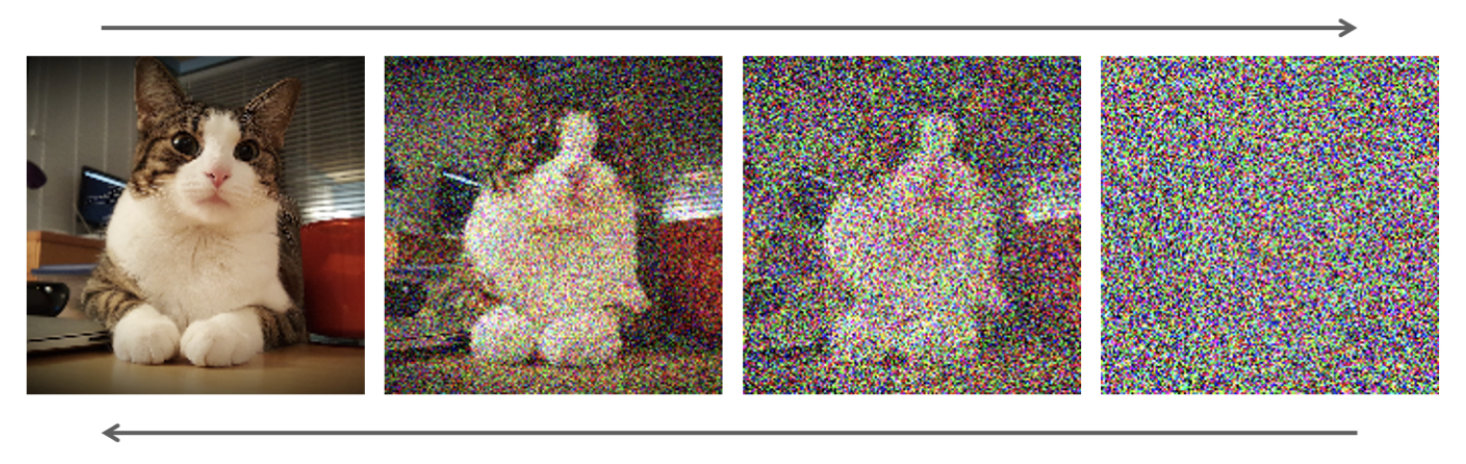
\includegraphics[width = 7in]{\images/DiffSequence}}

\vfill
{\huge
\centerline{{\color{red} [Sally talked to John]} $\stackrel{\rightarrow}{\leftarrow}$ {\color{red} [Sally talked to]}
$\stackrel{\rightarrow}{\leftarrow}$ {\color{red}[Sally talked]} $\stackrel{\rightarrow}{\leftarrow}$ {\color{red}[Sally]} $\stackrel{\rightarrow}{\leftarrow}$ {\color{red} []}}
}

\vfill
\centerline{$y \stackrel{\rightarrow}{\leftarrow} z_1  \stackrel{\rightarrow}{\leftarrow} \cdots \stackrel{\rightarrow}{\leftarrow} z_N$}

\slide{Hierarchical VAEs}
\centerline{$y \stackrel{\rightarrow}{\leftarrow} z_1  \stackrel{\rightarrow}{\leftarrow} \cdots \stackrel{\rightarrow}{\leftarrow} z_N$}

\vfill
{\bf Encoder}: $\pop(y)$, $P_\enc(z_1|y)$,$P_\enc(z_2|z_1),\ldots,P(z_N|z_{N-1})$.


\vfill
{\bf Generator}: $P_\pri(z_N),P_\dec(z_{N-1}|z_N),\ldots,P_\dec(z_1|z_2),P_\dec(y|z_1)$

\vfill
The encoder and the decoder define distributions
$P_\enc(y,z_1,\ldots,z_N)$ and $P_\gen(y,z_1,\ldots,z_N)$ respectively.

\slide{Hierarchical ELBO Loss}

\begin{eqnarray*}
H(y) & = & E_{(y,z_1,\ldots,z_n) \sim
P_\enc}\left[- \ln\frac{P_\gen(y,z_1,\ldots,z_n)}{P_\enc(z_1,\ldots,z_N|y)}\right]\\
\end{eqnarray*}

\slide{EM-VAEs}

The use of minimal encoder training may reflect the mode collapse problem of training a sampling distribution, such as a GAN generator or a VAE encoder.

\vfill
The situation might be different if a better method were available for training the encoder.
Here I will propose a method for training the encoder that avoids the mode collapse problem.

\slide{EM-VAEs}
We start with the following ``optimum encoder'' inequality.

\vfill
{\color{red}
$$E_{y \sim \pop,z \sim P_\gen(z|y)}\left[ - \ln \frac{P_\gen(y,z)}{P_\gen(z|y)}\right] \leq E_{(y,z) \sim P_\enc}\left[ - \ln \frac{P_\gen(y,z)}{P_\enc(z|y)}\right]$$
}

\vfill
This implies $P_\enc^*(z|y) = P_\gen(z|y)$ and universality gives


{\color{red} $$\enc^* = \argmin_\enc E_{(y,z) \sim P_\gen} -\ln P_\enc(z|y)$$}

\slide{EM-VAE}

\begin{eqnarray*}
\mbox{E:}\;\enc^* & = & {\color{red} \argmin_\enc E_{(y,z) \sim P_\gen} -\ln P_\enc(z|y)} \\
\\
\mbox{M:}\;\gen^* & =& {\color{red} \argmin_{\gen}\;E_{(y,z) \sim P_\enc(y,z)}\left[-\ln P_\gen(y,z)\right]}
\end{eqnarray*}

\vfill
The classical EM algorithm is the case where we alternate optimizing the encoder (the E step)
and the generator (the M step) and where the E step yields $P_\enc(z|y) = P_\gen(z|y)$ exactly
and where the $M$ step cannot fully fit the population.

\vfill
Here we can use SGD on these two objectives
independent of details of the models.

\slide{Derivation of the Encoder Optimum}

{\color{red} \Large
\begin{eqnarray*}
& & E_{(y,z) \sim P_\enc}\left[ - \ln \frac{P_\gen(y,z)}{P_\enc(z|y)}\right] \\
\\
& = & E_{(y,z) \sim P_\enc}\left[ - \ln \frac{P_\gen(y,z)}{P_\gen(z|y)}\right] + E_{y \sim \pop} \;KL(P_\enc(z|y),P_\gen(z|y)) \\
\\
& \geq & E_{(y,z) \sim P_\enc}\left[ - \ln \frac{P_\gen(y,z)}{P_\gen(z|y)}\right] \\
\\
& = & E_{(y,z) \sim P_\enc}\left[ - \ln P_\gen(y)\right] \\
\\
& = & E_{y \sim \pop,z \sim P_\gen(z|y)}\left[ - \ln P_\gen(y) \right]\\
\\
& = & E_{y \sim \pop,z \sim P_\gen(z|y)}\left[ - \ln \frac{P_\gen(y,z)}{P_\gen(z|y)}\right]
\end{eqnarray*}
}


\slide{END}

\end{document}


